\begin{definition}[Medians of a Triangle]
The medians of a triangle are the three segments going from each vertex to the midpoint of the opposite side.
\end{definition}

\begin{theorem}[Length of the Median in a Right Triangle]
In a right triangle, the length of the median drawn from the vertex of the right angle equals half the length of the triangle's hypotenuse.
\end{theorem}
\begin{figure}[H]
\centering
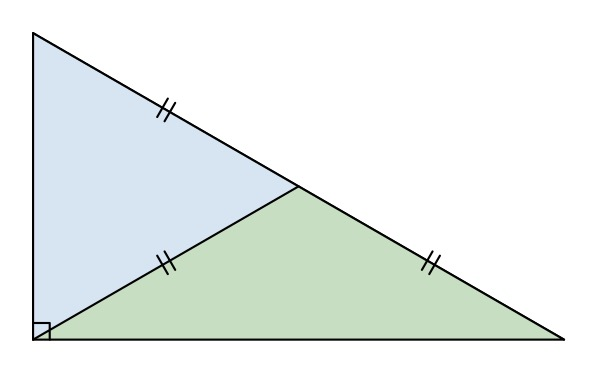
\includegraphics[height=5cm]{triangle-right-median}
\end{figure}
The median drawn from the vertex of the right angle always splits the right triangle into two isosceles triangles.
